% arara: pdflatex
%Began 24 April 2025 --- 
\documentclass[a4paper,x11names,svgnames,10pt]{article}
\usepackage{amsmath}
\usepackage{hyperref}
% the \hypersetup{keyvals} commented out below is stored in an external hyperref.cfg file
% to enable the pagebackref=true option
%\hypersetup{%dvips, % not needed for  pdflatex
%	pagebackref=true,
%	pdfauthor={Iam The Author},
%	hyperfigures,
%	bookmarks=true,
%	bookmarksnumbered=true,
%	bookmarksopen=true,
%	colorlinks=true, %if true, link borders absent
%	pdfborder={1 1 1},
%	citecolor=blue,
%	linkcolor=blue,
%	urlcolor=blue,
%}
\usepackage{url}
\usepackage{svg}
\usepackage[utf8]{inputenc}
\usepackage{graphicx}
\usepackage{xcolor}
\usepackage{float}
\usepackage{natbib}

\topmargin -0.50in
\oddsidemargin 0.0in
\textwidth 6.27in
\textheight 9.75in

%%%-----------------------------------------------------
%%% TO BE EDITED FOR EACH NEW SERIES or VOLUME GENERATED 
%%%-----------------------------------------------------
	\def\authorName{I Am The Author}
	\def\authorFirstMidNameInit{I.\ T.\ }
	\def\authorLastName{Author}
	\def\dateGenerated{\today}
	\def\volNumber{I}
	\def\mdgBookTitle{Musical Dice Game - \\[0.15cm] Minuets \volNumber}
	\def\mdgBookSubTitle{{\small based on}\\ Ludus Melothedicus ou \\[0.15cm] le Jeu de Dez Harmonique  }
	\def\theBookSeries{Wonders of the Musical World Series 8}
	\def\theBookPublisher{Libre Edition Press}
	\def\theBookPublisherLogo{../images/1ed.png}
	\def\theBookFrontCover{../images/FrontCover.pdf}
%%%-----------------------------------------------------
%%%

\def\uline{\underline}
%\definecolor{orange}{rgb}{1,0.5,0} % RGB
%\definecolor{light-gray}{gray}{0.95} % shades
%\definecolor{orange}{cmyk}{0,0.5,1,0} % CMYK

\newcommand{\HRule}{\rule{\linewidth}{0.5mm}}

\setlength{\parindent}{0pt}

\DeclareGraphicsExtensions{.pdf,.png}

\setcitestyle{authoryear,round,comma,aysep={,},yysep={,},notesep={, }}

\title{\textsc{\mdgBookTitle}}
\author{\textsc{\authorFirstMidNameInit \authorLastName}}
\date{\textsc{\dateGenerated}}
% ---

\begin{document}

% Book Cover
% File name: mdgBooSVG8v1-cover.tex
% Purpose: Book Cover
% Instruction: Should be \input{.} just after \begin{document}
{
\topmargin 0.00in
\oddsidemargin 0.45in
\textwidth 8.27in %letterpaper: 8.50in
\textheight 11.69in %letterpaper: 11.50in
\thispagestyle{empty}

\begin{titlepage}

\begin{picture}(0,0)%
\linethickness{70.00pt}
\color{blue!22!black}
\put(-105,85){\line(1,0){6477}}
\put(-105,-735){\includegraphics[clip=true,trim=0.0in 0.65in 0.25in 0.90in,height=12.50in,width=8.60in,keepaspectratio]	{\theBookFrontCover}}
\put(-105,-692){\line(1,0){6477}}
\end{picture}

\vspace{-1.5in}

\begin{center}
	\LARGE\textbf{\color{white} \hspace{-0.5in}\theBookSeries}
\end{center}


\vspace*{4.00\baselineskip}
\begin{center} \Huge\textbf{\color{MediumBlue!1!MidnightBlue}\em \mdgBookTitle}
\end{center}

\vspace{-0.20in}
\begin{center}
	\Large\textbf{\color{MediumBlue!50!MidnightBlue}\em \mdgBookSubTitle}
\end{center}

\begin{center}
	\LARGE\textbf{\color{MediumBlue!25!MidnightBlue}\em compiled by \authorFirstMidNameInit \authorLastName}
\end{center}

\vfill
\begin{center}
	\LARGE\textbf{\hspace{-0.5in}\color{white}\em \theBookPublisher \\ \vspace{-.19in}}
\end{center}
\end{titlepage}
}




\newpage
% Title Page
{
${}_{}$\\
\vspace{1.00in}	
\thispagestyle{empty}
\begin{center}
	\HRule \\[0.4cm]
	{\huge \bfseries \mdgBookTitle} \\[0.2cm]
	{\large{\em \mdgBookSubTitle} }\\[0.2cm]
	\HRule \\[1.5cm]
	% Author and supervisor
	\begin{minipage}{0.4\textwidth}
		\begin{flushleft} \large
			\emph{Author:}\\
			\authorFirstMidNameInit \textsc{\authorLastName}
		\end{flushleft}
	\end{minipage}
	\begin{minipage}{0.4\textwidth}
		\begin{flushright} \large
			\emph{Supervisor:} \\
			Dr. Communio \textsc{Sanctorum}
		\end{flushright}
	\end{minipage}
	\vfill
	% Bottom of the page
	{\textsc{\Large \theBookSeries}}  \\[0.2cm] 
	\includegraphics*[width=0.15\linewidth]{\theBookPublisherLogo}\\ 
	{\large \theBookPublisher \\
       \dateGenerated }\\
	\vspace{2.50in}
\end{center}
\newpage

%\maketitle		% uncomment if no Front Cover

\tableofcontents\label{tabofcon}

%\extrafloats{182}

\baselineskip 14pt

\newpage
\section[Introduction]{Introduction\footnote{The information contained in the introduction were culled from the following online resources:
		\href{https://imslp.org/wiki/Ludus_Melothedicus_(Anonymous)}{\it Ludus Melothedicus, ou Le eu de Dez Harmonique, 2nd ed. (1759)}, 
		\citet{wiki_mw2017},
		\url{https://opus-infinity.org/}, and 
		\href{https://www.sciencenews.org/article/mozarts-melody-machine-0}{Mozart's Melody Machine} \citep*{peterson2001}
	}
}
\begin{center}
	\begin{minipage}{0.4\textwidth}
		\begin{flushleft}
			\begin{center}
				``\small LUDUS MELOTHEDICUS OU \\ LE JEU DE DEZ HARMONIQUE \\
				Contenat plusieurs Calculs \\
				Par lesquels toute personne \\ Composera differents Menuets \\ 
				avec l'accompagnement de Basse  \\
				en jouant avec de deux Dez meme  \\
				sans scavior la Musique"
			\end{center}
		\end{flushleft}
	\end{minipage}
	\begin{minipage}{0.4\textwidth}
		\begin{flushright}
			\begin{center}
				``\small LUDUS MELOTHEDICUS OR \\ THE HARMONIC GAME OF DICE \\
				Containing several Calculations \\ 
				By which any person will \\
				Compose different Minuets \\ 
				with Bass accompaniment \\
				while playing with two Dice themselves \\ 
				without knowing Music."
			\end{center}
		\end{flushright}
	\end{minipage}
\end{center}

Thus run the French title and corresponding English translation of the Musical Dice Game (MDG) that was anonymously authored and was published by Chevardi\'{e}re: Paris in 1759 (\citealp{ludus1759}).  Rightly and interestingly so, as the Rules provided in this work allow a non-professional musician to generate (``compose") nearly two quadrillions ($2 \times 10^{12}$) of unique MDG minuets.  More precisely, the total number of minuets that the rules of the \href{https://imslp.org/wiki/Ludus_Melothedicus_(Anonymous)}{{\em Ludus Melothedicus}}, as we would refer to this MDG from here onward, yield is: $$9^{16} = 1\!,853\!,020\!,188\!,851\!,841.$$ 
Of these, $\mathbf{(9^6\times 8\times 7) \times (9^7\times 6) = 854\!,066\!,918\!,318\!,544}$ are unique since three pairs of measures for Part I and three pairs of measures for Part II are identical (see Section~\ref{genMeas} for more details).\\

\noindent A {\it Musikalisches W\"{u}rfelspiel} (German for ``musical dice game" or MDG) is a system for randomly ``generating" (e.g., by using a die or two dice) musical compositions from precomposed options and was quite popular throughout Western Europe in the 18th century.  The earliest known MDG is Johann Philipp Kirnberger's {\em Der allezeit fertige Polonoisen- und Menuettencomponist (1st ed.\ 1757; rev.\ 2nd ed.\ 1783)} (translated from German as ``The Ever-Ready Minuet and Polonaise Composer").  Other well-known composers that are to known to have composed a MDG are C.P.E.\ Bach ({\em Einfall, einen doppelten Contrapunct in der Octave von sechs Tacten zu machen, ohne die Regeln davon zu wissen (1758)}; translated from German as ``A method for making six bars of double counterpoint at the octave without knowing the rules"), Abb\'{e} Maximillian Stadler ({\em Table pour composer des minuets et des Trios \`{a} la infinie; avec deux dez \`{a} jouer (1780)}; translated from French as ``A table for composing minuets and trios to infinity, by playing with two dice"), the latter MDG being also attributed to Franz Joseph Haydn.\\

Probably the most famous of MDGs is {\it Musikalisches W\"{u}rfelspiel K. 516f (1787)}.  This MDG was first published by J.J. Hummel in 1793 in Berlin and was republished in 1796 by Nikolaus Simrock in Bonn (as K. 294d or K. Anh. C 30.01). Simrock attributed this work to Wolfgang Amadeus Mozart. It is also known under the title of {\em Anleitung zum Componieren von Walzern so viele man will vermittelst zweier W\"{u}rfel, ohne etwas von der Musik oder Composition zu verstehen} (German for ``Instructions for the composition of as many waltzes as one desires with two dice, without understanding anything about music or composition") and may have been based on Mozart's manuscript {\em K.\ 516f}, written in 1787, consisting of numerous two-bar fragments of music, that appear to be some kind of game or system for constructing music out of two-bar fragments, but contains no instructions nor hints as to the use of dice.  An \href{(http://www.asahi-net.or.jp/\~rb5h-ngc/e/k516f.htm}{online article} by Hideo Noguchi offers a possible explanation for this attribution.\\

For this book, we generate MDG minuets based on the rules given in the second edition of \href{https://imslp.org/wiki/Ludus_Melothedicus_(Anonymous)}{{\em Ludus Melothedicus}}.  Fifty (50) such MDG minuets are given toward the latter part of this book. The scores of these generated minuets were initially written using the \texttt{abc} environment of Chris Walshaw, then converted to Scalar Vector Graphics (SVG) images (with corresponding MIDIs) using {\tt abcm2ps} and {\tt abcmidi}, and then pre-processed with Inkscape to be included in \LaTeX\ to produce this book.


\section{\em Ludus Melothedicus}

\subsection{Rules}\label{mdgRules}

The Rules provided in \href{https://imslp.org/wiki/Ludus_Melothedicus_(Anonymous)}{{\em Ludus Melothedicus}} generate minuets consisting of 16 bars/measures that may be divided into two parts of eight bars each. Each part is played with a repeat. All told, a total of $16 \times 2 \;=\; 32$ bars of music is played for each minuet. \\

The notes for each bar of the minuet are determined by rolling a nine-sided top or die 16 times to get a sequence of integers whose terms are elements of the set \{1, 2, 3, 4, 5, 6, 7, 8, 9\}. The first eight toss outcomes will be used to create the eight bars of Part I of the minuet, latter eight toss outcomes to create the eight bars of Part II of the minuet, according to the rules given below (not exactly the same as given in the \href{https://imslp.org/wiki/Ludus_Melothedicus_(Anonymous)}{{\em Ludus Melothedicus}} as here, the Table of Measures for Parts I and II have already been constructed before hand; see Section~\ref*{genMeas} for more information). 

\begin{enumerate}
	\item [1.\label{step1}] To generate the notes for each of the eight bars of Part I of the minuet, simply look up the bar corresponding to the toss outcome (rows) and the current minuet bar number (column) in the Tables of Measures for Part I (Tables~\ref{fig:meas1} and \ref{fig:meas2}).  
	
	\item [2.\label{step2}] Similarly, to generate the notes for each of the eight bars of Part II of the minuet, repeat Step 1 but this time using the Tables of Measures for Part II (Tables~\ref{fig:meas3} and \ref{fig:meas4}). 
\end{enumerate}   

For example, if we are in the process of creating the fifth bar (Bar 5) of Part I of the minuet and the dice outcome was a 3, then we would use the notes in bar number 21 of Figure~\ref{fig:meas1}: {\tt [V:1] =B2G2=e2} for the G-clef and {\tt [V:2] G,2G,2G,2} for the F-clef. \\

The suggested accompaniments are a violin for the G-clef and bass or cello for the F-clef.


\subsection{How to Generate the Table of Measures}\label{genMeas}

To generate the Table of Measures ($(9\times 8) \times 2 = 144; 144 \times 2 = 288$ bars in all, since there are nine (9) possible die rolls, eight (8) bars for each part, two clefs (G and F) per part, and two parts: I and II) shown in Figure~\ref{fig:meas1}, \ref{fig:meas2}, \ref{fig:meas3}, and \ref{fig:meas4}, these measures being that for minuets in the Key of D, the notes (drawn in clefs) given in pages 6 (G-clef) and 7 (F-clef) , and the tables for note numbers given in pages 8 to 11 of \href{https://imslp.org/wiki/Ludus_Melothedicus_(Anonymous)}{{\em Ludus Melothedicus}} are used. \\  

For example if a 2 is rolled for the first bar, then we use the table of note numbers given on page 8 of \href{https://imslp.org/wiki/Ludus_Melothedicus_(Anonymous)}{{\em Ludus Melothedicus}} (this particular table is reproduced below with annotations on how to obtain the note numbers that are to be used to find the notes from those given on pages 6 and 7; see Figure~\ref{fig:r2m1}).  Since we rolled a 2, we start at the first box (containing 66) and count this as the 3rd box, then count until the ninth box to land on the box containing 108, and use this as the first note number.  We then take the numbers in every ninth box thereafter until there are no more boxes to be counted, keeping in mind that on even rows we go from right to left, we skip empty boxes, and that 0s are simply disregarded.  When two numbers appear in a box, e.g., 75/71, two notes are obtained and a double string is played. \\  

Hence, when a 2 is rolled for the first bar of Part I of the minuet to be written in the Key of D, the note numbers to be used are: 108, 103, 190, 108, 113, 195, 111, 114, and 189.  Looking at the G- and F-clefs on pages 6 and 7 of \href{https://imslp.org/wiki/Ludus_Melothedicus_(Anonymous)}{{\em Ludus Melothedicus}}, we obtain the notes (in {\tt abc} notation): {\tt [V:1] dAd$^\wedge$f=eg} and {\tt [V:2] D,2$^\wedge$F,2$^\wedge$C,2}, where notes corresponding to note numbers less than 120 are assigned to the violin ({\tt [V:1]}) and notes corresponding to note numbers greater than 119 are assigned to the bass/cello ({\tt [V:2]}).  In addition, whenever there is an excess of obtained notes to a bar, a succession of three (3) half notes may have to be played as a triplet or an eight note may have to be played as a grace note.

\begin{table}[H]
	\centering
	\begin{tabular}{c}
		\centering
		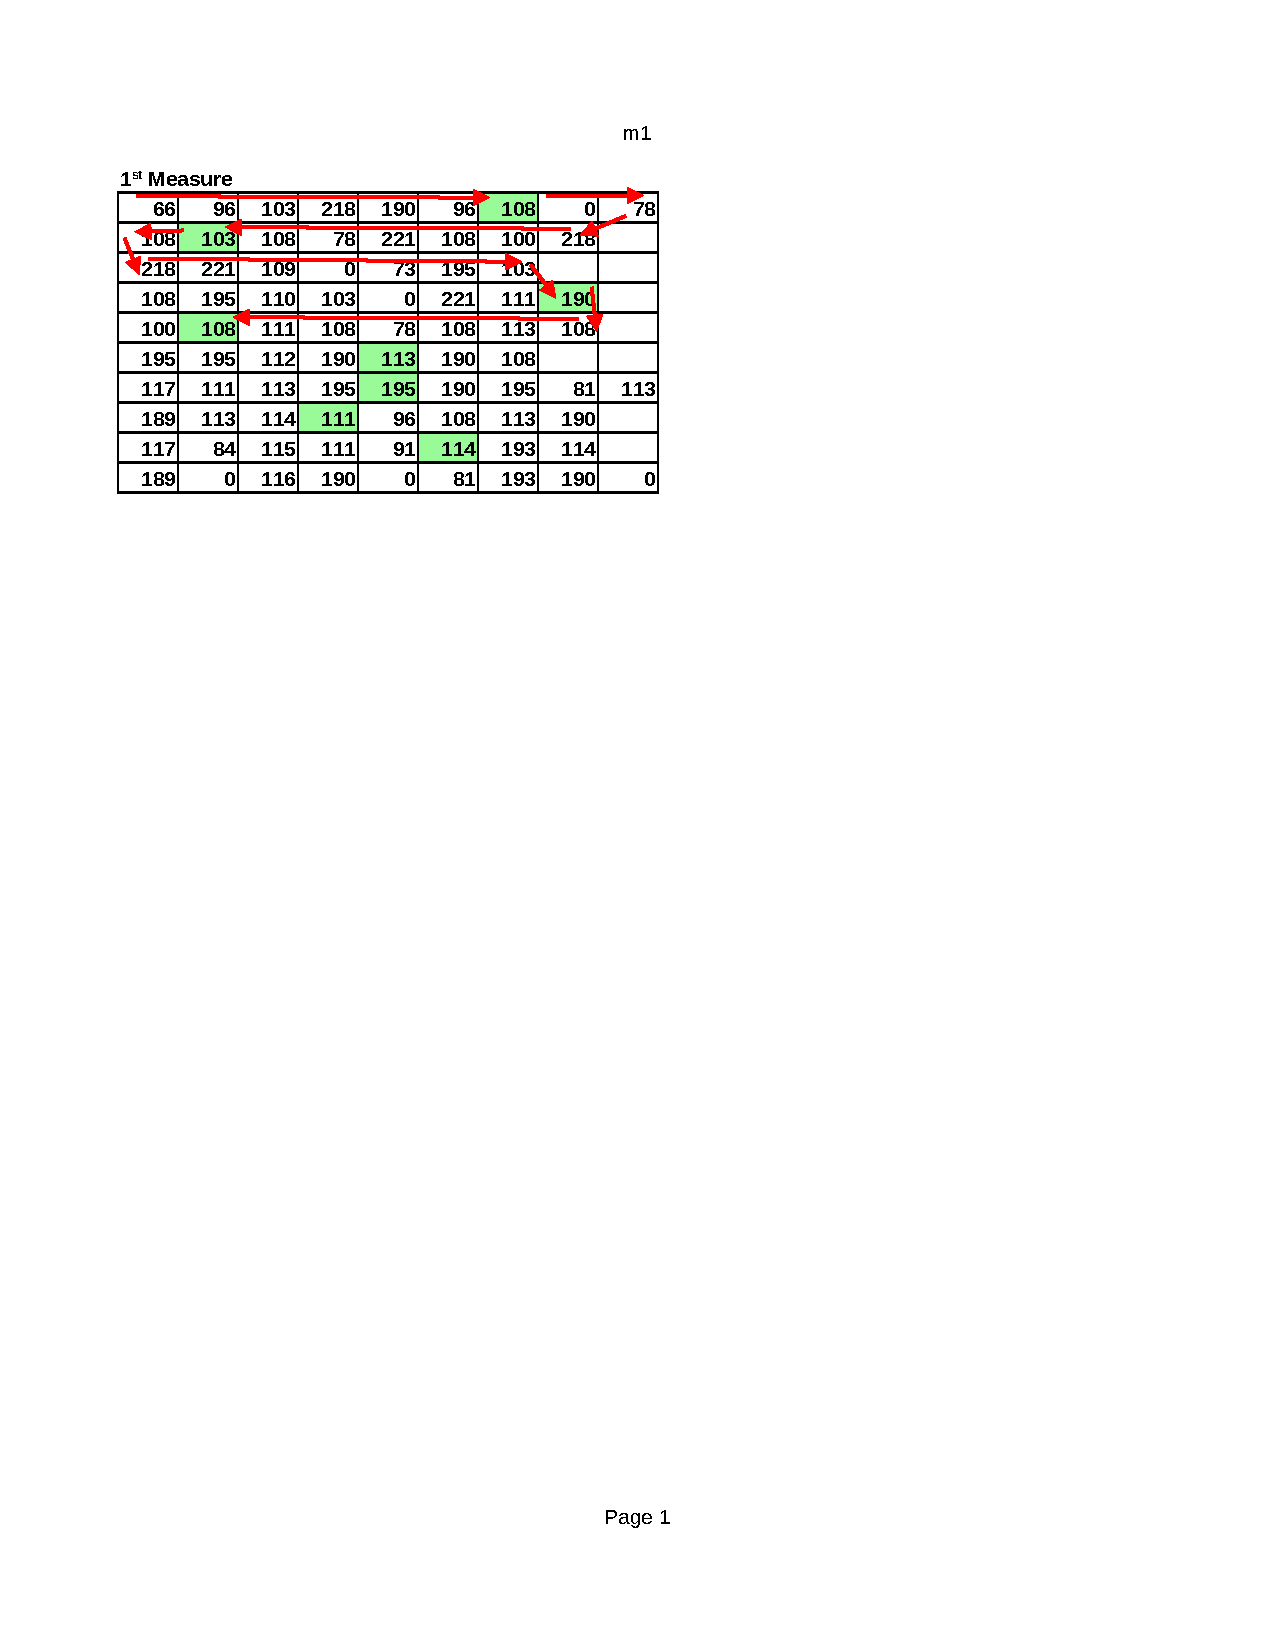
\includegraphics[clip=true,trim=0.75in 7.60in 4.00in 1.10in,scale=0.90]{ludus9-D-m1}
	\end{tabular}
	\caption{Table of note numbers to be used when a 2 is rolled for bar 1, Part I of minuets in the Key of D.  Thus when a 2 is rolled for the first bar of Part I of the minuet, the note numbers of the notes to be used are: 108, 103, 190, 108, 113, 195, 111, 114, and 189 (box highlighted with light green). The notes corresponding to these note numbers are obtained from the G- and F-clefs given in pages 6 and 7 of \href{https://imslp.org/wiki/Ludus_Melothedicus_(Anonymous)}{{\em Ludus Melothedicus}}. These yield the notes (in {\tt abc} notation): {\tt [V:1] dAd$^\wedge$f=eg} and {\tt [V:2] D,2$^\wedge$F,2$^\wedge$C,2}.}
	\label{fig:r2m1}
\end{table}

Additional examples are given in pages 4 and 5 of \href{https://imslp.org/wiki/Ludus_Melothedicus_(Anonymous)}{{\em Ludus Melothedicus}}.  These are summarized in Tables~\ref{tab:ex1} and \ref{tab:ex2} below.

\begin{table}[H]
	\centering
	\begin{tabular}{|c|c|l|} \hline
		\tt Bar & \tt Roll & \tt Note Numbers for Notes to be Used (Part I))\\ \hline\hline
		\tt 1 & \tt 2 & \tt 108, 103, 190, 108, 113, 195, 111, 114, and 189 \\ \hline
		\tt 2 & \tt 8 & \tt 114, 24, 190, 0, 189, 81, 0, 185,  and 0 \\ \hline
		\tt 3 & \tt 3 & \tt 113, 117, 190, 195, 114, 111, 196, 105, and 111 \\ \hline
		\tt 4 & \tt 2 & \tt 77, 105, 107, 198, 73, 196, 195, and 0  \\ \hline
		\tt 5 & \tt 9 & \tt 233, 228, 224, 223, 17, 114, 113, 111, and 193 \\ \hline
		\tt 6 & \tt 7 & \tt 108, 19, 233, 230, 226, 224, 78, 223, and 218 \\ \hline
		\tt 7 & \tt 9 & \tt 111, 103, 84, 189, 113, 114, 117, 193, and 190 \\ \hline 
		\tt 8 & \tt 2 & \tt 0, 0, 198, 51, 193, 185, and 0 \\ \hline\hline
	\end{tabular}
	\caption{Examples for obtaining note numbers for the eight bars of Part I of the minuet in the Key of D (see page 4 of \href{https://imslp.org/wiki/Ludus_Melothedicus_(Anonymous)}{{\em Ludus Melothedicus}}). Note that 0s are disregarded when looking up for notes.}
	\label{tab:ex1}
\end{table}

\begin{table}[H]
	\centering
	\begin{tabular}{|c|c|l|} \hline
		\tt Bar & \tt Roll & \tt Note Numbers for Notes to be Used (Part II)\\ \hline\hline
		\tt 1 & \tt 5 & \tt 27, 190, 195, 113, 103, 0, 190, 0, and 0 \\ \hline
		\tt 2 & \tt 5 & \tt 105, 101, 196, 100, 96, 190, 71, and 183  \\ \hline
		\tt 3 & \tt 3 & \tt 105, 111, 114, 119, 196, 232, 196, 0, and 78 \\ \hline
		\tt 4 & \tt 4 & \tt 107, 111, 102, 198, 193, 185, 15, and 0  \\ \hline
		\tt 5 & \tt 6 & \tt 75, 233, 224, 0, 221, 218, 25, 217, and 215 \\ \hline
		\tt 6 & \tt 9 & \tt 108, 19, 233, 226, 78, 224, 226, 223, and 218 \\ \hline
		\tt 7 & \tt 8 & \tt 105, 103, 101, 140, 100, 98, 96, 198, 95, 96, and 98 \\ \hline 
		\tt 8 & \tt 7 & \tt 190, 233, 217, 213, 217, 37, and 0 \\ \hline\hline
	\end{tabular}
	\caption{Examples for obtaining note numbers for the eight bars of Part II of the minuet in the Key of D (see page 5 of \href{https://imslp.org/wiki/Ludus_Melothedicus_(Anonymous)}{{\em Ludus Melothedicus}}). Note that 0s are disregarded when looking up for notes.}
	\label{tab:ex2}
\end{table}

\subsection{Table of Measures}\label{tabMeas}

The Table of Measures for Part I of the minuets based on \href{https://imslp.org/wiki/Ludus_Melothedicus_(Anonymous)}{{\em Ludus Melothedicus}} are given in Figures~\ref{fig:meas1} and  \ref{fig:meas2}, that follow while that for Part II are given in Tables~\ref{fig:meas3} and \ref{fig:meas4}.  The notes of the bars in these four tables were generated based on \href{https://imslp.org/wiki/Ludus_Melothedicus_(Anonymous)}{\href{https://imslp.org/wiki/Ludus_Melothedicus_(Anonymous)}{{\em Ludus Melothedicus}}}.

%\newpage
${}_{}$\\
\vspace{0.10in}
\addcontentsline{toc}{subsection}{\hspace*{0.25in} {\em Ludus Melothedicus - Part I} of measures (page 1/2)}	
\begin{figure}[H]
	\centering
	\def\svgwidth{0.975\columnwidth}
	\input{ludus-part1-D001.pdf_tex}
	\caption{Table of Measures - Part I (Page 1/2)}
	\label{fig:meas1}
\end{figure}

\newpage
${}_{}$\\
\vspace{0.10in}
\addcontentsline{toc}{subsection}{\hspace*{0.25in} {\em Ludus Melothedicus - Part I} of measures (page 2/2)}	
\begin{figure}[H]
	\centering
	\def\svgwidth{0.975\columnwidth}
	\input{ludus-part1-D002.pdf_tex}
	\caption{Table of Measures - Part I (Page 2/2)}
	\label{fig:meas2}
\end{figure}

${}_{}$\\
\vspace{0.10in}
\addcontentsline{toc}{subsection}{\hspace*{0.25in} {\em Ludus Melothedicus - Part II} of measures (page 1/2)}	
\begin{figure}[H]
	\centering
	\def\svgwidth{0.975\columnwidth}
	\input{ludus-part2-D001.pdf_tex}
	\caption{Table of Measures - Part II (Page 1/2)}
	\label{fig:meas3}
\end{figure}

\newpage
${}_{}$\\
\vspace{0.10in}
\addcontentsline{toc}{subsection}{\hspace*{0.25in} {\em Ludus Melothedicus - Part II} of measures (page 2/2)}	
\begin{figure}[H]
	\centering
	\def\svgwidth{0.975\columnwidth}
	\input{ludus-part2-D002.pdf_tex}
	\caption{Table of Measures - Part II (Page 2/2)}
	\label{fig:meas4}
\end{figure}

Note that except for Bars 4 and 8 for Part I, there are nine (9) possible choices for measures to be played.  Furthermore, 
\begin{enumerate}
	\item for Bar 4 of Part I, the notes for die rolls 2 and 3 are the same.
	\item for Bar 8 of Part I, the notes for die rolls 1 and 5, and those for rolls 2 and 7 are the same.
\end{enumerate}
Thus, for Bar 4 of Part I has only 8 choices for bars to be played and Bar 8 of Part I has only 7 such choices. \\

For Part II, the first seven bars each have nine (9) possible choices for measures to be played.  Bar 8 (final bar) of Part II has three pairs of identical measures: Bars 1 and 6 are the same, as are Bars 2 and 7, and Bars 4 and 9.  These yield only six (6) possible choices for measures to be played for Bar 8, Part II. All told, the total number of unique MDG minuets based on \href{https://imslp.org/wiki/Ludus_Melothedicus_(Anonymous)}{\it Ludus Melothedicus} is equal to $$\underbrace{(9^6\times 8\times 7)}_{\text{Part I}} \times \underbrace{(9^7\times 6)}_{\text{Part II}} = 854\!,066\!,918\!,318\!,544.$$

%\newpage
\section{Related Links}
The following are very interesting sites in that they allow the online rendering of MDGs:
\begin{itemize}
	\item \href{https://opus-infinity.org}{Opus Infinity} - Collaborative work of Robbert Harms, Hein Moors, and Suus van Petegem whose goal is to unravel the mystery behind the tables used for generating MDGs.  Site visitors can generate MDGs based on works of Kirnberger, Mozart, Stadler/Haydn, Bach, Gerlach, and Callegari ({\it 1st Cahier}).  Corresponding audio files ({\tt mid, ogg,} and/or {\tt mp3}) and image files ({\tt pdf} or {\tt png}) are also made available for listening, viewing, or downloading.
	
	\item  \href{http://sunsite.univie.ac.at/Mozart/dice/}{Mozart} - A site maintained by John Chuang that allows the site visitor to generate MDGs based on the work of Stadler/Haydn.
	
	\item  \href{https://marian-aldenhoevel.de/mozart/}{Mozart} - A site maintained by Marian Aldenh\"{o}vel allows the visitor to generate a MDG (user-specified or randomly-generated) and the corresponding audio ({\tt midi, wav}) and image files ({\tt pdf, png}) based on {\em Musikalisches W\"{u}rferspiel, K.\ 516f}.
	
	\item \href{https://www.amaranthpublishing.com/mozart.zip}{\tt mozart.zip} -  This is a Windows software ({\small\textcopyright} 1995 VisionSoft) by John Chuang and Stephen Goodwin that generates MDG based on input from user and is available for {\it free} from  \href{http://www.amaranthpublishing.com/MozartDiceGame.htm}{Amaranth Publishing}.  
	
	\item \href{(http://www.asahi-net.or.jp/\~rb5h-ngc/e/k516f.htm}{``Mozart - Musical Game in C K. 516f,"}	Mozart Studies Online - The site of Hideo Noguchi that offers an explanation linking {\em Musikalisches W\"{u}rferspiel, K.\ 516f}, and  {\em K.\ 294d (K.\ Anh.\ C 30.01)}. 
\end{itemize}

\newpage
\section{Acknowledgments}
Special thanks to \href{https://imslp.org}{International Music Score Library Project} for \href{https://imslp.org/wiki/Ludus_Melothedicus_(Anonymous)}{\it Ludus Melothedicus, ou Le Jeu de Dez Harmonique, 2nd ed. (1759)}, \href{https://opus-infinity.org}{Opus Infinity} for additional related information, and \href{http://www.amaranthpublishing.com/MozartDiceGame.htm}{Amaranth Publishing} for a copy of {\tt mozart.zip}. My sincerest gratitude to Chris Walshaw et al. for the \href{http://www.abcnotation.com/}{ABC music notation}; Jean-Francois Moine for \href{http://moinejf.free.fr/}{\tt abcm2ps} and the accompanying examples, templates, and pointers for the appropriate use of these resources; Guido Gonzato for the \href{http://abcplus.sourceforge.net/}{ABC Plus Project} and the \href{http://abcplus.sourceforge.net/#abcMIDI}{{\tt abcmidi} resources} available there, more especially for the ABC resource book {\em Making Music with ABC 2}; James R. Allwright and Seymour Shlien for \href{http://abc.sourceforge.net/abcMIDI}{\tt abcmidi} source and binaries; \href{https://artifex.com/}{Artifex, Inc.} for Ghostscript v.10.00.0 (includes the {\tt ps2pdf} converter); \href{https://www.inkscape.org/}{Inkscape v.1.2.2} for the tool for converting SVGs to PDFs for inclusion into \LaTeX\ documents; William Schelter for \href{https://maxima.sourceforge.io}{Maxima v.5.47.0}---used for computing the permutation number; \href{https://google.lens}{Google Lens} and \href{https://translate.google.com}{Google Translate} for aiding in producing the English versions of the text of \href{https://imslp.org/wiki/Ludus_Melothedicus_(Anonymous)}{{\em Ludus Melothedicus}}; Colomban Wendling et.\ al for \href{https://www.geany.org}{Geany 2.0 IDE}; and \href{https://tex.stackexchange.com/users/632/martin-h}{\tt User:Martin H} for his \href{https://tex.stackexchange.com/questions/2099/how-to-include-svg-diagrams-in-latex}{reply} to a \TeX\ / \LaTeX\ Stack Exchange question on including SVGs into \LaTeX\ documents. Thanks to  Ditto to Machtelt Garrels for the book \href{http://tldp.org/LDP/Bash-Beginners-Guide/html/Bash-Beginners-Guide.html}{Bash Guide for Beginners}, Vivek Gite for the book \href{http://www.freeos.com/guides/lsst/}{Linux Script Shell Tutorial}, and Steve Parker for the \href{http://steve-parker.org/sh/cheatsheet.pdf}{Unix/Linux Shell Cheatsheet}. John Fogarty's GitHub Site: \href{https://github.com/jfogarty/latex-createspace-bookcover}{Latex CreateSpace BookCover} and Peter Wilson's reply in  \TeX\ / \LaTeX\ Stack Exchange on \href{https://tex.stackexchange.com/questions/17579/how-can-i-design-a-book-cover}{designing a book cover}, were sources of ideas, information, and materials for creating the book cover and title page, thanks to both of them; \href{http://www.libreoffice.org/}{LibreOffice Calc} for its use in the image creation of the book cover.  Many thanks, too, to the \href{https://www.debian.org}{Debian Project} for the Debian 12 (Bookworm) GNU/Linux OS, \href{http://www.tug.org/texlive/}{TeXLive} for providing the \TeX\ distribution,  and \href{https://github.com}{GitHub} for its generosity in providing space for \href{https://github.com/justineuro/mdgBookSVG8Kit}{the project}.  

%\newpage
\section{Fifty (50) Selected Minuets based on \href{https://imslp.org/wiki/Ludus_Melothedicus_(Anonymous)}{{\em Ludus Melothedicus}}}
%\vspace{-.10in}
This section contains an example of 50 minuets that were generated using the Rules in Section~\ref{mdgRules}. 
\vspace{0.20in}
{
	\topmargin -0.25in
	\textheight 9.25in
	\input{svgList}
}	

%\newpage
\vspace{0.25in}
\section{License}
This work by I Am The Author, based on work of J.L.A. Uro at \url{https://github.com/justineuro/mdgBookSVG8Kit}, is licensed under a Creative Commons Public Domain International License.

\bibliographystyle{plainnat}
\bibliography{mdg8}



\end{document}
